\documentclass{article}

\edef\restoreparindent{\parindent=\the\parindent\relax}

\usepackage[utf8]{inputenc}
\usepackage[dutch]{babel}
\usepackage[parfill]{parskip}
\usepackage{enumerate}
\usepackage{amsthm, amssymb, mathtools, amsmath}
\usepackage[margin=3cm]{geometry}
\usepackage[hidelinks]{hyperref}

\restoreparindent

\newcommand{\p}{\mathbb{P}}
\newcommand{\e}{\mathbb{E}}
\renewcommand{\r}{\mathbb{R}}
\newcommand{\f}{\mathcal{F}}
\renewcommand{\lim}[2]{\underset{#1\to#2}{\text{lim}}}
\newcommand{\liminfty}[1]{\lim{#1}{\infty}}
\newcommand{\defeq}{\vcentcolon=}

\newcommand{\avg}[1]{\overline{#1}}

\DeclareMathOperator{\mse}{MSE}

\DeclareMathOperator{\unif}{Uniform}
\DeclareMathOperator{\expon}{Exponentieel}
\DeclareMathOperator{\bin}{Binomiaal}
\DeclareMathOperator{\var}{Var}
\DeclareMathOperator{\cov}{Cov}

\title{Samenvatting Stochastiek 2}
\author{Jonas van der Schaaf}
\date{\today}

\begin{document}
\maketitle
\tableofcontents

\newpage
\section{Introductie}

<<<<<<< HEAD
\subsection{De verzameling $\mathbb{R}$}
\paragraph{Algebraïsche eigenschappen}De verzameling breuken $\mathbb{Q}$ heeft de volgende algebraïsche eigenschappen:
\begin{itemize}
    \setlength\itemsep{0em}
    \item[\textbf{A1.}] $a+(b+c)=(a+b)+c$ voor elke $a,b,c\in\mathbb{Q}$.
    \item[\textbf{A2.}] $a+b=b+a$ voor alle $a,b\in\mathbb{Q}$.
    \item[\textbf{A3.}] $a+0=0$ voor alle $a\in\mathbb{Q}$.
    \item[\textbf{A4.}] Voor elke $a\in\mathbb{Q}$ is er een $-a\in\mathbb{Q}$ zodat $a+(-a)=0$
    \item[\textbf{M1.}] $a(bc)=(ab)c$ voor elke $a,b,c\in\mathbb{Q}$.
    \item[\textbf{M2.}] $ab=ba$ voor alle $a,b\in\mathbb{Q}$.
    \item[\textbf{M3.}] $a\cdot1=a$ voor alle $a\in\mathbb{Q}$.
    \item[\textbf{M4.}] Voor elke $a\in\mathbb{Q}$ met $a\neq0$ is er een $a^{-1}\in\mathbb{Q}$ zodat $a \cdot a^{-1} = 1$
\end{itemize}
De eigenschappen \textbf{A1} en \textbf{M1} zijn de \textit{associatieve} eigenschappen van $+$ en $\cdot$ en de eigenschappen \textbf{A2} en \textbf{M2} zijn de \textit{commutatieve} eigenschappen van $+$ en $\cdot$.

\subparagraph{Consequenties van de veld eigenschappen} De volgende eigenschappen volgen uit de algebraïsche eigenschappen van $\mathbb{Q}$:

\begin{enumerate}
    \setlength\itemsep{0em}
    \item Als $a+c=b+c$ dan geldt dat $a=b$.
    \item $a\cdot0=0$ voor alle $a\in\mathbb{Q}$.
    \item $(-a)b=-ab$ voor alle $a,b\in\mathbb{Q}$.
    \item $(-a)(-b)=ab$ voor alle $a,b\in\mathbb{Q}$.
    \item Als $ac=bc$ en $c\neq0$ dan $a=b$.
    \item Als $ab=0$ dan geldt dat $a=0$ of $b=0$.
\end{enumerate}
\textit{De bewijzen van deze stellingen staan op pagina 16 van het boek.}

\paragraph{Ordening}Ook heeft $\mathbb{Q}$ een ordening \bq$\leq$\eq die aan de volgende eigenschappen voldoet:
\begin{itemize}
    \setlength\itemsep{0em}
    \item[\textbf{O1.}] Als $a,b\in\mathbb{Q}$ dan geldt dat $a \leq b$ of $b \leq a$.
    \item[\textbf{O2.}] Als $a \leq b$ en $b \leq a$ dan $a=b$.
    \item[\textbf{O3.}] Als $a \leq b$ en $b \leq c$ dan $a \leq c$.
    \item[\textbf{O4.}] Als $a \leq b$ dan geldt ook dat $a+c \leq b+c$
    \item[\textbf{O5.}] Als $a \leq b$ en $c \geq 0$, dan ook $ac \leq bc$.
\end{itemize}
De eigenschap \textbf{O3} heet de \textit{transitieve} eigenschap. Een veld met een ordening die voldoet aan \textbf{O1} tot en met \textbf{O5} heet een geordend veld.

\subparagraph{Consequenties van de ordening ''$\leq$''}
\begin{enumerate}
    \setlength\itemsep{0em}
    \item Als $a \leq b$ dan $-b \leq -a$.
    \item Als $a \leq b$ en $c\leq0$ dan $bc \leq ac$.
    \item Als $0 \leq a$ en $0 \leq b$ dan $0 \leq ab$.
    \item $0 \leq a^{2}$ voor elke $a\in\mathbb{Q}$.
    \item $0<1$.
    \item Als $0 < a$ dan ook $0 < a^{-1}$.
    \item Als $0<a<b$ dan geldt $0<b^{-1}<a^{-1}$.
\end{enumerate}
\textit{Dit wordt bewezen op pagina 16-17 van het boek.}

\paragraph{Absolute waarde} De absolute waarde is gedefinieerd als volgt:
$$
|a|\defeq
\begin{cases}
    a & \text{als } a\geq 0\\
    -a & \text{als } a<0
\end{cases}
$$
\subparagraph{Stellingen over de absolute waarde} De volgende stellingen over de absolute waarde zijn waar:
\begin{enumerate}
    \setlength\itemsep{0em}
    \item $|a|\geq0$.
    \item $|ab|=|a|\cdot|b|$.
    \item $|a+b|\leq|a|+|b|$.
\end{enumerate}
\textit{Dit wordt bewezen op pagina 17-18 van het boek.}

\paragraph{Afstand} De afstand tussen twee getallen $a,b$ is de $\text{dist}(a,b)$ wat gedefiniëerd is als:
$$\text{dist}(a,b)\defeq|a-b|$$
\paragraph{Stellingen over de afstand} De volgende stelling over afstand is waar:

\subparagraph{Afstand tussen de som van getallen} $\text{dist}(a,c)\leq\text{dist}(a,b)+\text{dist}(b,c)$.

\textit{Dit wordt bewezen op pagina 18 van het boek.}

\paragraph{Stellingen uit opgaven} De volgende handige stellingen worden bewezen in een opgave uit paragraaf $3$:

\subparagraph{Opgave 3.5a} Voor elke $a,b\in\mathbb{R}$ geldt dat $|b| \leq a$ dan en slechts dan als $-a \leq b \leq a$.

\subparagraph{Opgave 3.5b} Voor elke $a,b\in\mathbb{R}$ geldt dat $||b|-|a|| \leq |b-a|$.

\subparagraph{Opgave 3.6b} Laat $a_{1},a_{2},...,a_{n}\in\mathbb{R}$, dan geldt dat $|\sum_{i=1}^{n}a_{i}|\leq\sum_{i=1}^{n}|a_{i}|$
\subsection{De compleetheid van \texorpdfstring{$\mathbb{R}$}{R}}

\paragraph{Maxima en minima} Van een verzameling $S\subseteq\mathbb{R}$ zijn het maximum en minimum als volgt gedefiniëerd:
\subparagraph{Maximum} $s_{0} = \text{max}(S)$ dan en slechts dan als voor elke $s \in S$ geldt dat $s \leq s_{0}$ en $s_{0} \in S$.
\subparagraph{Minimum}$s_{0} = \text{min}(S)$ dan en slechts dan als voor elke $s \in S$ geldt dat $s \geq s_{0}$ en $s_{0} \in S$.

\paragraph{Intervallen} Een interval is een speciaal soort deelverzameling van $\mathbb{R}$, er zijn 4 verschillende intervallen:
\begin{itemize}
    \setlength\itemsep{0em}
    \item $[a,b]\defeq\{x\in\mathbb{R}:a \leq x \leq b\}$ dit heet een gesloten interval. $\text{min}([a,b])=a$ en $\text{max}([a,b])=b$.
    \item $[a,b)\defeq\{x\in\mathbb{R}:a \leq x < b\}$ dit heet een half gesloten interval. $\text{min}([a,b))=a$ en $\text{max}([a,b))$ bestaat niet.
    \item $(a,b]\defeq\{x\in\mathbb{R}:a < x \leq b\}$ dit heet een half gesloten interval. $\text{min}((a,b])=a$ en $\text{max}((a,b])$ bestaat niet.
    \item $(a,b)\defeq\{x\in\mathbb{R}:a < x < b\}$ dit heet een open interval. $\text{min}((a,b))$ bestaat niet en $\text{max}((a,b))$ bestaat niet.
\end{itemize}

\paragraph{Boven- en ondergrenzen} Boven- en ondergrenzen zijn als volgt gedefiniëerd: Laat $S\subseteq\mathbb{R}$ dan geldt

\subparagraph{Bovengrens} Een getal $M$ is een bovengrens van $S$ als voor elke $s \in S$ geldt dat $s \leq M$. Als een verzameling een bovengrens heeft dan heet die verzameling boven begrensd.

\subparagraph{Ondergrens} Een getal $m$ is een ondergrens van $S$ als voor elke $s \in S$ geldt dat $s \geq m$. Als een verzameling een ondergrens heeft dan heet die verzameling onder begrensd.

\paragraph{Stellingen over boven- en ondergrenzen} De volgende stelling wordt gegeven over bovengrenzen:

\subparagraph{Intervallen en begrenzingen} Als $S$ boven en beneden begrensd is, dan zijn er twee getallen $m,M\in\mathbb{R}$ zodat $S\subseteq [m,M]$.

\paragraph{Suprema en infima} Het supremum en infimum van een verzameling zijn als volgt gedefiniëerd:

\subparagraph{Supremum} $M=\text{sup}(S)$ dan en slechts dan als voor elke $s \in S$ geldt dat $s \leq M$ en voor elke $M_{1}<M$ geldt dat er een $s \in S$ is zodat $M_{1}<s$. Dan is $M$ de kleinste bovengrens van $S$.

\subparagraph{Infimum} $m=\text{inf}(S)$ dan en slechts dan als voor elke $s \in S$ geldt dat $m \geq s$ en voor elke $m>m_{1}$ geldt dat er een $s \in S$ waarvoor geldt dat $s<m$. Dan is $m$ de grootste ondergrens van $S$.

\paragraph{Stellingen} In paragraaf 4 van hoofdstuk 1 staan de volgende stellingen:

\subparagraph{Volledigheidsaxioma van $\mathbb{R}$} Het volledigheidsaxioma luidt als volgt: Voor elke $S\subseteq\mathbb{R}$ met $S\neq\emptyset$ met een bovengrens is er een $M\in\mathbb{R}$ zodat $M=\text{sup}(S)$. \textit{Dit is een axioma, er is geen bewijs.}

\subparagraph{``Omgekeerde'' volledigheids \bq axioma\eq} Voor elke $S\in\mathbb{R}$ met $S\neq\emptyset$ met een ondergrens is er een $m\in\mathbb{R}$ zodat $m=\text{inf}(S)$. Het is geen echt axioma want het volgt uit het volledigheidsaxioma. \textit{Het bewijs staat op pagina 24-25 van het boek.}

\subparagraph{Archimedische eigenschap} Zij $a,b\in\mathbb{R}^{+}$ met $a<b$. Dan geldt dat er een $n\in\mathbb{N}$ zodat $na>b$. \textit{Het bewijs staat op pagina 25 van het boek.}

\subparagraph{De dichtheid van $\mathbb{Q}$} Als $a,b\in\mathbb{R}$ en $a<b$ dan is er een $r\in\mathbb{Q}$ zodat $a<r<b$. \textit{Het bewijs staat op pagina 25-26 van het boek.}

\paragraph{Stellingen uit opgaven} De volgende stellingen worden bewezen in een opgave uit paragraaf $4$:

\subparagraph{Opgave 4.7a} Laat $S$ en $T$ verzamelingen zijn met $S,T\subseteq\mathbb{R}$ zodat $S \subseteq T$. Dan geldt dat $\text{inf}(T)\leq\text{inf}(S)\leq\text{sup}(S)\leq\text{sup}(T)$.

\subparagraph{Opgave 4.7b} Laat $S$ en $T$ verzamelingen zijn met met $S,T\subseteq\mathbb{R}$. Dan geldt dat $\text{sup}(S \cup T) = \text{max}\{\text{sup}(S), \text{sup}(T)\}$.

\subparagraph{Opgave 4.8b} Laat $S$ en $T$ verzamelingen zijn zodat voor elke $s \in S$ en $t \in T$ geldt dat $s \leq t$. Dan geldt dat $\text{sup}(S)\leq\text{inf}(T)$.

\subparagraph{Opgave 4.9} Laat $S$ een verzameling zijn zodat $S\subseteq\mathbb{R}$, dan geldt dat $\text{inf}(S)=-\text{sup}(-S)$.

\subparagraph{Opgave 4.14a} Laat $A$ en $B$ verzamelingen zijn met $A,B\subseteq\mathbb{R}$ en $A+B=\{a+b:a \in A \text{ en } b \in B\}$. Dan geldt dat $\text{sup}(A+B)=\text{sup}(A)+\text{sup}(B)$.

\subparagraph{Opgave 4.14b} Laat $A$ en $B$ verzamelingen zijn met $A,B\subseteq\mathbb{R}$. Dan geldt dat $\text{inf}(A+B)=\text{inf}(A)+\text{inf}(B)$.

=======
\subsection{De verzameling $\mathbb{R}$}
\paragraph{Algebraïsche eigenschappen}De verzameling breuken $\mathbb{Q}$ heeft de volgende algebraïsche eigenschappen:
\begin{itemize}
    \setlength\itemsep{0em}
    \item[\textbf{A1.}] $a+(b+c)=(a+b)+c$ voor elke $a,b,c\in\mathbb{Q}$.
    \item[\textbf{A2.}] $a+b=b+a$ voor alle $a,b\in\mathbb{Q}$.
    \item[\textbf{A3.}] $a+0=0$ voor alle $a\in\mathbb{Q}$.
    \item[\textbf{A4.}] Voor elke $a\in\mathbb{Q}$ is er een $-a\in\mathbb{Q}$ zodat $a+(-a)=0$
    \item[\textbf{M1.}] $a(bc)=(ab)c$ voor elke $a,b,c\in\mathbb{Q}$.
    \item[\textbf{M2.}] $ab=ba$ voor alle $a,b\in\mathbb{Q}$.
    \item[\textbf{M3.}] $a\cdot1=a$ voor alle $a\in\mathbb{Q}$.
    \item[\textbf{M4.}] Voor elke $a\in\mathbb{Q}$ met $a\neq0$ is er een $a^{-1}\in\mathbb{Q}$ zodat $a \cdot a^{-1} = 1$
\end{itemize}
De eigenschappen \textbf{A1} en \textbf{M1} zijn de \textit{associatieve} eigenschappen van $+$ en $\cdot$ en de eigenschappen \textbf{A2} en \textbf{M2} zijn de \textit{commutatieve} eigenschappen van $+$ en $\cdot$.

\subparagraph{Consequenties van de veld eigenschappen} De volgende eigenschappen volgen uit de algebraïsche eigenschappen van $\mathbb{Q}$:

\begin{enumerate}
    \setlength\itemsep{0em}
    \item Als $a+c=b+c$ dan geldt dat $a=b$.
    \item $a\cdot0=0$ voor alle $a\in\mathbb{Q}$.
    \item $(-a)b=-ab$ voor alle $a,b\in\mathbb{Q}$.
    \item $(-a)(-b)=ab$ voor alle $a,b\in\mathbb{Q}$.
    \item Als $ac=bc$ en $c\neq0$ dan $a=b$.
    \item Als $ab=0$ dan geldt dat $a=0$ of $b=0$.
\end{enumerate}
\textit{De bewijzen van deze stellingen staan op pagina 16 van het boek.}

\paragraph{Ordening}Ook heeft $\mathbb{Q}$ een ordening \bq$\leq$\eq die aan de volgende eigenschappen voldoet:
\begin{itemize}
    \setlength\itemsep{0em}
    \item[\textbf{O1.}] Als $a,b\in\mathbb{Q}$ dan geldt dat $a \leq b$ of $b \leq a$.
    \item[\textbf{O2.}] Als $a \leq b$ en $b \leq a$ dan $a=b$.
    \item[\textbf{O3.}] Als $a \leq b$ en $b \leq c$ dan $a \leq c$.
    \item[\textbf{O4.}] Als $a \leq b$ dan geldt ook dat $a+c \leq b+c$
    \item[\textbf{O5.}] Als $a \leq b$ en $c \geq 0$, dan ook $ac \leq bc$.
\end{itemize}
De eigenschap \textbf{O3} heet de \textit{transitieve} eigenschap. Een veld met een ordening die voldoet aan \textbf{O1} tot en met \textbf{O5} heet een geordend veld.

\subparagraph{Consequenties van de ordening ''$\leq$''}
\begin{enumerate}
    \setlength\itemsep{0em}
    \item Als $a \leq b$ dan $-b \leq -a$.
    \item Als $a \leq b$ en $c\leq0$ dan $bc \leq ac$.
    \item Als $0 \leq a$ en $0 \leq b$ dan $0 \leq ab$.
    \item $0 \leq a^{2}$ voor elke $a\in\mathbb{Q}$.
    \item $0<1$.
    \item Als $0 < a$ dan ook $0 < a^{-1}$.
    \item Als $0<a<b$ dan geldt $0<b^{-1}<a^{-1}$.
\end{enumerate}
\textit{Dit wordt bewezen op pagina 16-17 van het boek.}

\paragraph{Absolute waarde} De absolute waarde is gedefinieerd als volgt:
$$
|a|\defeq
\begin{cases}
    a & \text{als } a\geq 0\\
    -a & \text{als } a<0
\end{cases}
$$
\subparagraph{Stellingen over de absolute waarde} De volgende stellingen over de absolute waarde zijn waar:
\begin{enumerate}
    \setlength\itemsep{0em}
    \item $|a|\geq0$.
    \item $|ab|=|a|\cdot|b|$.
    \item $|a+b|\leq|a|+|b|$.
\end{enumerate}
\textit{Dit wordt bewezen op pagina 17-18 van het boek.}

\paragraph{Afstand} De afstand tussen twee getallen $a,b$ is de $\text{dist}(a,b)$ wat gedefiniëerd is als:
$$\text{dist}(a,b)\defeq|a-b|$$
\paragraph{Stellingen over de afstand} De volgende stelling over afstand is waar:

\subparagraph{Afstand tussen de som van getallen} $\text{dist}(a,c)\leq\text{dist}(a,b)+\text{dist}(b,c)$.

\textit{Dit wordt bewezen op pagina 18 van het boek.}

\paragraph{Stellingen uit opgaven} De volgende handige stellingen worden bewezen in een opgave uit paragraaf $3$:

\subparagraph{Opgave 3.5a} Voor elke $a,b\in\mathbb{R}$ geldt dat $|b| \leq a$ dan en slechts dan als $-a \leq b \leq a$.

\subparagraph{Opgave 3.5b} Voor elke $a,b\in\mathbb{R}$ geldt dat $||b|-|a|| \leq |b-a|$.

\subparagraph{Opgave 3.6b} Laat $a_{1},a_{2},...,a_{n}\in\mathbb{R}$, dan geldt dat $|\sum_{i=1}^{n}a_{i}|\leq\sum_{i=1}^{n}|a_{i}|$
\subsection{De compleetheid van \texorpdfstring{$\mathbb{R}$}{R}}

\paragraph{Maxima en minima} Van een verzameling $S\subseteq\mathbb{R}$ zijn het maximum en minimum als volgt gedefiniëerd:
\subparagraph{Maximum} $s_{0} = \text{max}(S)$ dan en slechts dan als voor elke $s \in S$ geldt dat $s \leq s_{0}$ en $s_{0} \in S$.
\subparagraph{Minimum}$s_{0} = \text{min}(S)$ dan en slechts dan als voor elke $s \in S$ geldt dat $s \geq s_{0}$ en $s_{0} \in S$.

\paragraph{Intervallen} Een interval is een speciaal soort deelverzameling van $\mathbb{R}$, er zijn 4 verschillende intervallen:
\begin{itemize}
    \setlength\itemsep{0em}
    \item $[a,b]\defeq\{x\in\mathbb{R}:a \leq x \leq b\}$ dit heet een gesloten interval. $\text{min}([a,b])=a$ en $\text{max}([a,b])=b$.
    \item $[a,b)\defeq\{x\in\mathbb{R}:a \leq x < b\}$ dit heet een half gesloten interval. $\text{min}([a,b))=a$ en $\text{max}([a,b))$ bestaat niet.
    \item $(a,b]\defeq\{x\in\mathbb{R}:a < x \leq b\}$ dit heet een half gesloten interval. $\text{min}((a,b])=a$ en $\text{max}((a,b])$ bestaat niet.
    \item $(a,b)\defeq\{x\in\mathbb{R}:a < x < b\}$ dit heet een open interval. $\text{min}((a,b))$ bestaat niet en $\text{max}((a,b))$ bestaat niet.
\end{itemize}

\paragraph{Boven- en ondergrenzen} Boven- en ondergrenzen zijn als volgt gedefiniëerd: Laat $S\subseteq\mathbb{R}$ dan geldt

\subparagraph{Bovengrens} Een getal $M$ is een bovengrens van $S$ als voor elke $s \in S$ geldt dat $s \leq M$. Als een verzameling een bovengrens heeft dan heet die verzameling boven begrensd.

\subparagraph{Ondergrens} Een getal $m$ is een ondergrens van $S$ als voor elke $s \in S$ geldt dat $s \geq m$. Als een verzameling een ondergrens heeft dan heet die verzameling onder begrensd.

\paragraph{Stellingen over boven- en ondergrenzen} De volgende stelling wordt gegeven over bovengrenzen:

\subparagraph{Intervallen en begrenzingen} Als $S$ boven en beneden begrensd is, dan zijn er twee getallen $m,M\in\mathbb{R}$ zodat $S\subseteq [m,M]$.

\paragraph{Suprema en infima} Het supremum en infimum van een verzameling zijn als volgt gedefiniëerd:

\subparagraph{Supremum} $M=\text{sup}(S)$ dan en slechts dan als voor elke $s \in S$ geldt dat $s \leq M$ en voor elke $M_{1}<M$ geldt dat er een $s \in S$ is zodat $M_{1}<s$. Dan is $M$ de kleinste bovengrens van $S$.

\subparagraph{Infimum} $m=\text{inf}(S)$ dan en slechts dan als voor elke $s \in S$ geldt dat $m \geq s$ en voor elke $m>m_{1}$ geldt dat er een $s \in S$ waarvoor geldt dat $s<m$. Dan is $m$ de grootste ondergrens van $S$.

\paragraph{Stellingen} In paragraaf 4 van hoofdstuk 1 staan de volgende stellingen:

\subparagraph{Volledigheidsaxioma van $\mathbb{R}$} Het volledigheidsaxioma luidt als volgt: Voor elke $S\subseteq\mathbb{R}$ met $S\neq\emptyset$ met een bovengrens is er een $M\in\mathbb{R}$ zodat $M=\text{sup}(S)$. \textit{Dit is een axioma, er is geen bewijs.}

\subparagraph{``Omgekeerde'' volledigheids \bq axioma\eq} Voor elke $S\in\mathbb{R}$ met $S\neq\emptyset$ met een ondergrens is er een $m\in\mathbb{R}$ zodat $m=\text{inf}(S)$. Het is geen echt axioma want het volgt uit het volledigheidsaxioma. \textit{Het bewijs staat op pagina 24-25 van het boek.}

\subparagraph{Archimedische eigenschap} Zij $a,b\in\mathbb{R}^{+}$ met $a<b$. Dan geldt dat er een $n\in\mathbb{N}$ zodat $na>b$. \textit{Het bewijs staat op pagina 25 van het boek.}

\subparagraph{De dichtheid van $\mathbb{Q}$} Als $a,b\in\mathbb{R}$ en $a<b$ dan is er een $r\in\mathbb{Q}$ zodat $a<r<b$. \textit{Het bewijs staat op pagina 25-26 van het boek.}

\paragraph{Stellingen uit opgaven} De volgende stellingen worden bewezen in een opgave uit paragraaf $4$:

\subparagraph{Opgave 4.7a} Laat $S$ en $T$ verzamelingen zijn met $S,T\subseteq\mathbb{R}$ zodat $S \subseteq T$. Dan geldt dat $\text{inf}(T)\leq\text{inf}(S)\leq\text{sup}(S)\leq\text{sup}(T)$.

\subparagraph{Opgave 4.7b} Laat $S$ en $T$ verzamelingen zijn met met $S,T\subseteq\mathbb{R}$. Dan geldt dat $\text{sup}(S \cup T) = \text{max}\{\text{sup}(S), \text{sup}(T)\}$.

\subparagraph{Opgave 4.8b} Laat $S$ en $T$ verzamelingen zijn zodat voor elke $s \in S$ en $t \in T$ geldt dat $s \leq t$. Dan geldt dat $\text{sup}(S)\leq\text{inf}(T)$.

\subparagraph{Opgave 4.9} Laat $S$ een verzameling zijn zodat $S\subseteq\mathbb{R}$, dan geldt dat $\text{inf}(S)=-\text{sup}(-S)$.

\subparagraph{Opgave 4.14a} Laat $A$ en $B$ verzamelingen zijn met $A,B\subseteq\mathbb{R}$ en $A+B=\{a+b:a \in A \text{ en } b \in B\}$. Dan geldt dat $\text{sup}(A+B)=\text{sup}(A)+\text{sup}(B)$.

\subparagraph{Opgave 4.14b} Laat $A$ en $B$ verzamelingen zijn met $A,B\subseteq\mathbb{R}$. Dan geldt dat $\text{inf}(A+B)=\text{inf}(A)+\text{inf}(B)$.

>>>>>>> 41d8c4ccd1df145e9b394c4ee2d5ea58fd90f71e

\section{Verdelingsonderzoek}
\subsection{Univariate steekproeven}
\paragraph{Steekproefgemiddelde} Het steekproefgemiddelde van een steekproef \(X_{1},\dots,X_{n}\) is de stochastische grootheid
\[
    \avg{X}=\frac{1}{n}\sum_{i=1}^{n}X_{i}.
\]

\paragraph{Steekproefvariantie} De steekproefvariantie van een steekproef \(X_{1},\dots,X_{n}\) is de stochastische grootheid
\[
    S_{X}^{2}=\frac{1}{n-1}\sum_{i=1}^{n}\left(X_{i}-\avg{X}\right)^{2}.
\]

\subsection{Histogrammen}
Zij \(X_{1},\dots,X_{n}\) een steekproef met bereik \(R\subseteq\r\) en \(a_{0}<\dots<a_{m}\) een partitie van \(R\). Dan is het histogram van de steekproef op een interval \((a_{j-1},a_{j}]\) gegeven door
\[
    h(x)=\frac{1}{a_{j}-a_{j-1}}\sum_{i=1}^{n}1_{(a_{j-1},a_{j}]}(x_{i}).
\]
Het geschaalde histogram schaalt het histogram met een factor \(\frac{1}{n}\). Het geschaalde histogram is dus gelijk aan
\[
    h(x)=\frac{1}{n(a_{j}-a_{j-1})}\sum_{i=1}^{n}1_{(a_{j-1},a_{j}]}(x_{i}).
\]

\subsection{Boxplots}
\paragraph{Kwartielen} Gegeven een steekproef \(X_{1},\dots,X_{n}\) is net \(n\)-de kwartiel de waarde \(X_{i}\) zodat precies \(\frac{n}{4}\) uitkomsten van de steekproef kleiner zijn dan \(X_{i}\).

\paragraph{Boxplots} Een boxplot is een grafiek waarin de kwartielen van een steekproef weergegeven zijn. Het boxplot van een normaalverdeling ziet er bij benadering uit als in figuur \ref{fig:boxplot_norm}.

\begin{figure}[ht]
    \centering
    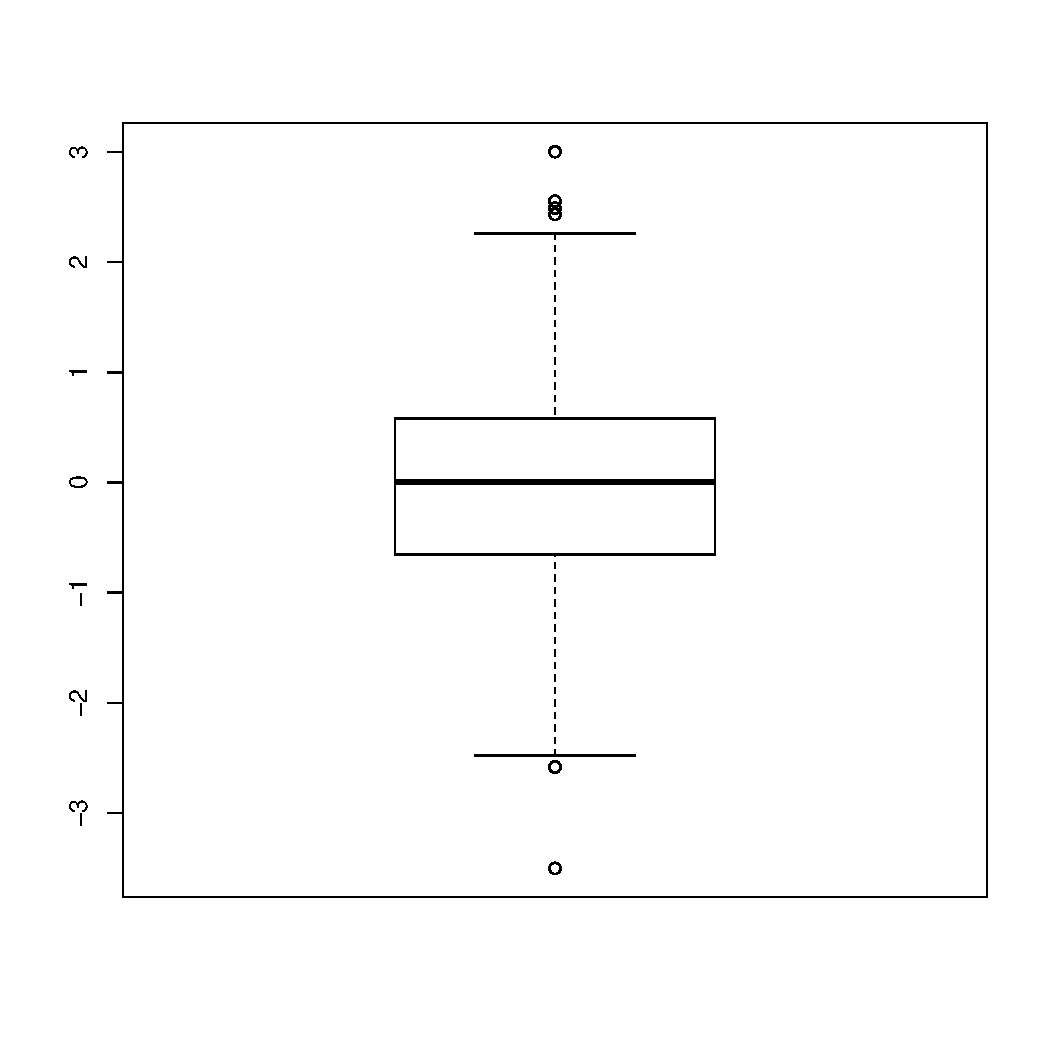
\includegraphics[width=0.7\textwidth]{plots/data.pdf}
    \caption{Een benadering van het boxplot van een normaalverdeling.}
    \label{fig:boxplot_norm}
\end{figure}

\subsection{Locatie schaalfamilie}
\paragraph{Locatie-schaalfamilie} Gegeven een stochastische grootheid \(X\) met verdelingsfunctie \(F\), dan heeft de stochast \(Y=a+bX\) de verdelingsfunctie \(F_{a,b}\) gegeven door
\[
    F_{a,b}(y)=\p(a+bX\leq y)=F\left(\frac{y-a}{b}\right).
\]
De familie kansverdelingen \(\{F_{a,b}\colon a\in\r,b>0\}\) heet de locatie-schaalfamilie behorend bij \(F\) of van \(X\).

\paragraph{Kwantielen} Gegeven een stochast \(X\) met verdelingsfunctie \(F\) is het \(\alpha\)-kwantiel (voor \(\alpha\in(0,1)\)) gelijk aan
\[
    F^{-1}(\alpha)=\inf\{x\colon F(x)\geq\alpha\}.
\]

\paragraph{Ordestatistieken} De ordestatistieken van een steekproef \(X_{1},\dots,X_{n}\) worden gegeven door de rij \(X_{(1)},\dots,X_{(n)}\) zodat ze geplaatst zijn in stijgende volgorde.

Voor de \(i\)-de ordestatistiek geldt dat \(\e F(X_{(i)})=\frac{i}{n+1}\) en algemener geldt dat \(X_{(i)}=a+bF^{-1}\left(\frac{i}{n+1}\right)\) voor \(X_{1},\dots,X_{n}\) elementen verdeeld met \(F_{a,b}\).

\paragraph{QQ-plot} Een QQ-plot van de data \(x_{1},\dots,x_{n}\) ten opzichte van een verdelingsfunctie \(F\) is een grafiek van de punten
\[
    \left\{\left(F^{-1}\left(\frac{i}{n+1}\right),x_{(i)}\right)\mid i=1,\dots,n\right\}.
\]

\subsection{Samenhang}
\paragraph{Scatterplot} Een scatterplot van tweedimensionale data \((x_{1},y_{1}),\dots,(x_{n},y_{n})\) is een grafiek van deze punten in het \(\r^{2}\)-vlak.

\paragraph{Steekproefcorrelatiecoëfficiënt} Het steekproefcorrelatiecoëfficiënt van een steekproef bestaande uit paren \((X_{1},Y_{1}),\dots,(X_{n},Y_{n})\) is
\[
    r_{X,Y}=\frac{\sum_{i=1}^{n}(X_{i}-\avg{X})(Y_{i}-\avg{Y})}{(n-1)\sqrt{S_{X}^{2}}\sqrt{S_{Y}^{2}}}.
\]

Het steekproefcorrelatiecoëfficiënt is een mate van lineairiteit van het verband tussen de waarden \(x_{i}\) en \(y_{i}\).

\paragraph{Auto-correlaties} Gegeven de uitkomst van een steekproef \(x_{1},\dots,x_{n}\) is het auto-correlatiecoëfficiënt een maat van correlatie tussen \(x_{i}\) en \(X_{i-h}\). Het wordt gegeven door
\[
    r_{x}(h)=\frac{\sum_{i=1}^{n-h}(x_{i+h}-\avg{x})(x_{i}-\avg{x})}{(n-h)s_{x}^{2}}.
\]
\section{Schatters}
\subsection{Eigenschappen van schatters}
\paragraph{Wat is een schatter} Een schatter of statistiek is een stochastische vector \(T(X)\) die alleen van \(X\) afhangt.

Als een kansverdeling van \(X\) afhangt van een parameter \(\theta\) zodat \(P_{\theta}\) de kansverdeling is van \(X\), dan is \(\theta\) vaak onbekend, dus dan worden schatters gebruikt om gegeven een realisatie van \(X\) de parameter \(\theta\) te schatten.

\paragraph{Mean Square Error} Gegeven een schatter \(T\) voor een de waarde van \(g(\theta)\), dan is de verwachte kwadratische fout van een schatter de waarde
\[
    \mse(\theta;T)=\e_{\theta}\left\|T-g(\theta)\right\|^{2}.
\]

De Mean Square Error kan ontbonden worden in twee termen:
\[
    \mse(\theta;T)=\var_{\theta}(T)+(\e T-g(\theta))^{2}.
\]

\paragraph{Niet-toelaatbare schatters} Gegeven twee schatters \(T_{1},T_{2}\) van een parameter \(\theta\) met voor elke \(\theta\in\Theta\), met \(\Theta\) de parameterruimte.
\[
    \e_{\theta}\left\|T_{1}-g(\theta)\right\|^{2}\leq\e_{\theta}\left\|T_{2}-g(\theta)\right\|^{2},
\]
dan heet \(T_{2}\) ontoelaatbaar.

\paragraph{Zuivere schatters} Gegeven een schatter \(T\) voor \(g(\theta)\), dan is de onzuiverheid van \(T\) gedefiniëerd als
\[
    \e_{\theta}(T)-g(\theta)=0.
\]
Een schatter is zuiver als voor elke \(\theta\in\Theta\) dat de onzuiverheid gelijk is aan \(0\).

\subsection{Maxmimum Likelihood-Schatters}
\paragraph{Likelihood-functie} Zij \(X\) een stochastische vector met een kansdichtheid \(p_{\theta}\) die afhangt van \(\theta\in\Theta\) met \(\Theta\) de parameterruimte. Dan is voor een vaste \(x\), de functie
\[
    \theta\mapsto L(\theta;x)=p_{\theta}(x),
\]
de likelihood-functie.

\paragraph{Maximum likelihood-schatter} Gegeven een likelihood-functie \(L\) voor een stochast \(X\), dan is de maximum likelihood-schatter \(T(X)\) de waarde voor \(\theta\) zodat \(p_{\theta}(x)\) maximaal is.

\subsection{Momentschatters}
\paragraph{Momenten van een stochast} Gegeven een stochastische variabele afhankelijk van een parameter \(\theta\), dan is het \(j\)-de moment het getal \(\e_{\theta}(X^{j})\), als deze verwachting bestaat.

\paragraph{Steekproefmoment} Gegeven een steekproef \(X_{1},\dots,X_{n}\), dan is het \(j\)-de steekproef moment gegeven door \(\avg{X^{j}}\).

\paragraph{Momentenschatter} Zij \(X_{1},\dots,X_{n}\) een steekproef met onbekende parameter \(\theta\). Dan is de momentschatter de waarde \(\hat{\theta}\) zodat \(\e_{\hat{\theta}}(X^{j})=\avg{X^{j}}\) voor de eerste \(n\) momenten zodat \(\hat{\theta}\) uniek bepaald is. Dat betekent in de praktijk vaak dat \(\hat{\theta}\) bepaald wordt door het eerste moment dat afhankelijk is van de parameter \(\theta\).

\subsection{Bayes-schatters}
Een bayes schatter is een schatter voor een parameter \(\theta\in\Theta\). Er wordt een a priori\footnote{Letterlijk van tevoren.} kansverdeling \(\pi\colon\Theta\to\r\) opgesteld voor \(\theta\), die aangeeft hoe waarschijnlijk een bepaalde waarde van een parameter is. Afhankelijk van de data wordt dan de kansverdeling aangepast tot een a posteriori\footnote{Letterlijk van later, beter vertaald als afgeleid uit de feiten.} kansverdeling.

\paragraph{Bayes-risico} Gegeven een a priori verdeling \(\pi\) is het Bayes-risico van een schatter \(T\) voor \(g(\theta)\) gedefiniëerd als
\[
    R(\theta;T)-\int\e_{\theta}\left(T-g(\theta)\right)^{2}\pi(\theta)\,d\theta.
\]

\paragraph{Bayes-schatter} Gegeven een a priori dichtheid \(\pi\) is de Bayes-schatter de schatter \(T\) die \(R(\theta;T)\) minimaliseert.

De expliciete formule voor de Bayes-schatter is
\[
    T(x)=\frac{\int g(\theta)p_{\theta}(x)\pi(\theta\,dx)}{\int p_{\vartheta}(x)\pi(\vartheta)\,d\vartheta}.
\]
In Bayesiaanse notatie wordt dit geschreven als
\[
    T(x)=\e\left(g\left(\overline{\Theta}\right)\mid X=x\right).
\]

\paragraph{A posteriori dichtheid} De a posteriori dichtheid van \(\overline{\Theta}\) is gelijk aan
\[
    p_{\overline{\Theta}\mid X=x}(\theta)=\frac{p_{\theta}(x)\pi(\theta)}{\int p_{\vartheta}(x)\pi(\vartheta)\,d\vartheta}.
\]
\section{Optimaliteitstheorie}
\subsection{Voldoende statistieken}
\paragraph{Voldoende voor discrete statistieken} Voor een statistisch model \(X\) bestaande uit discrete verdelingen afhankelijk van parameter \(\theta\) heet een statistiek \(V=V(X)\) voldoende als
\[
    \p(X=x\mid V=v)
\]
onafhankelijk is van \(\theta\) voor alle \(x\) en \(v\).
\paragraph{Factorisatiestelling voor discrete voldoende statistieken}  Een statistisch model \(X\) bestaande uit discrete verdelingen afhankelijk van parameter \(\theta\) heet voldoende precies als
\[
    p_{\theta}(x)=g_{\theta}(V(x))h(x)
\]
voor twee functies \(g_{\theta}\) en \(h\) voor alle \(x\) en \(\theta\).

\paragraph{Voldoende continue statistieken} Een statistiek \(V(X)\) heet voldoende voor een waarneming \(X\) precies als er functies \(g_{\theta}\) en \(h\) zijn zodat voor alle \(\theta\) en \(x\) geldt dat
\[
    p_{\theta}(x)=g_{\theta}(V(x))h(x).
\]
Dit is voor discrete verdelingen precies de definitie, maar voor continue verdelingen geeft dit nu ook een definitie.

\subparagraph{Functies van statistieken} Zij \(V\) een voldoende statistiek en \(V^{*}\) een statistiek zodat \(V=f(V^{*})\), dan is \(V^{*}\) ook voldoende.

\subsection{Schattingstheorie}
\paragraph{Verschillende criteria voor schatters} Er zijn heel veel verschillende manieren om een bepaalde schatter te kiezen boven een andere. Hier volgen een paar:
\subparagraph{Bayes-criterium} Gegeven een a priori dichtheid \(\pi\) op \(\Theta\) is het Bayes-criterium het criterium dat de schatter \(T\) boven \(T'\) verkiest als
\[
    \int \mse(\theta;T)\pi(\theta)\,d\theta\leq\int \mse(\theta;T')\pi(\theta)\,d\theta.
\]
De schatter \(T\) die dit criterium minimaliseert is precies de Bayes schatter.

\subparagraph{Minimax criterium} Het minimax criterium verkiest een schatter \(T\) boven \(T'\) als
\[
    \sup_{\theta\in\Theta}\mse(\theta; T)\leq\sup_{\theta\in\Theta}\mse(\theta;T').
\]

\subsection{UMVZ-schatters}
\paragraph{UMVZ-schatter} Een schatter \(T\) heet uniform minimum variantie zuiver (UMVZ) als \(T\) zuiver is voor \(g(\theta)\) en \(\var_{\theta}(T)\leq\var_{\theta}(S)\) voor alle \(\theta\) en alle zuivere schatters \(S\) voor \(g(\theta)\).

\paragraph{Rao-Blackwell} Zij \(V=V(X)\) een voldoende statistiek en \(T=T(X)\) een willekeurige schatter voor \(g(\theta)\). Dan is er een schatter \(T^{*}\) die alleen afhankelijk is van \(V\) met \(\e_{\theta}T=\e_{\theta}T^{*}\) en \(\var_{\theta}T^{*}\leq\var_{\theta}T\). Bovendien geldt dat \(\mse(\theta;T^{*})\leq\mse(\theta;T)\), met de ongelijkheid strict als \(\p_{\theta}(T^{*}=T)=1\).

\paragraph{Volledige statistiek} Een statistiek \(V\) heet volledig precies als, als geldt dat \(\e_{\theta}(f(V))=0\) dan geldt dat \(\p_{\theta}(f(V)=0)\).

\paragraph{Voldoende, volledig en UMVZ} Zij \(V\) een voldoende en volledige statistiek en \(T=V(T)\) een zuivere schatter voor \(g(\theta)\). Dan is \(T\) een UMVZ-schatter voor \(g(\theta)\).

\paragraph{Exponentiële familie} Een familie kansdichtheden \(p_{\theta}\) heet een \(k\)-dimensionele familie als er functies \(c\), \(h\), \(Q_{j}\) en \(V_{j}\) bestaan zodat
\[
    p_{\theta}(x)=c(\theta)h(x)e^{\sum_{j}^{k}Q_{j}(\theta)V_{j}(x)}.
\]

\paragraph{Exponentiële familie, voldoende en volledig} Gegeven een \(k\)-dimensionele exponentiële familie \(p_{\theta}\). Dan is \(V=(V_{1},\dots,V_{n}\) voldoende en volledig als de verzameling \(\{(Q_{1}(\theta),\dots,Q_{n}(\theta)\mid\theta\in\Theta\}\) een inwendig punt heeft.
\end{document}